\documentclass[a4paper]{article}
\usepackage[top=1in, bottom=1.25in, left=1.25in, right=1.25in]{geometry}
\usepackage{amsmath}
\usepackage{multicol}
\usepackage{graphicx}
\RequirePackage{ltxcmds}[2010/12/07]
%opening
\title{M-QAM Mapper}

\begin{document}
	
\maketitle

This block does the mapping of the binary signal using a \textit{m}-QAM modulation. It atributes to each pair of bits a point in the I-Q space. The constellation is defined by the \textit{iqAmplitudes} vector.

\subsection*{Input Parameters}

\begin{itemize}
	\item m 
	\item iqAmplitudes 
\end{itemize}

\subsection*{Functional Description}



\subsection*{Input Signals}

\textbf{Number}: 1

\textbf{Type}: Binary (DiscreteTimeDiscreteAmplitude)

\subsection*{Output Signals}

\textbf{Number}: 2

\textbf{Type}: Sequence of 1's and -1's (DiscreteTimeDiscreteAmplitude)

\subsection*{Examples}

\begin{figure}[h]
	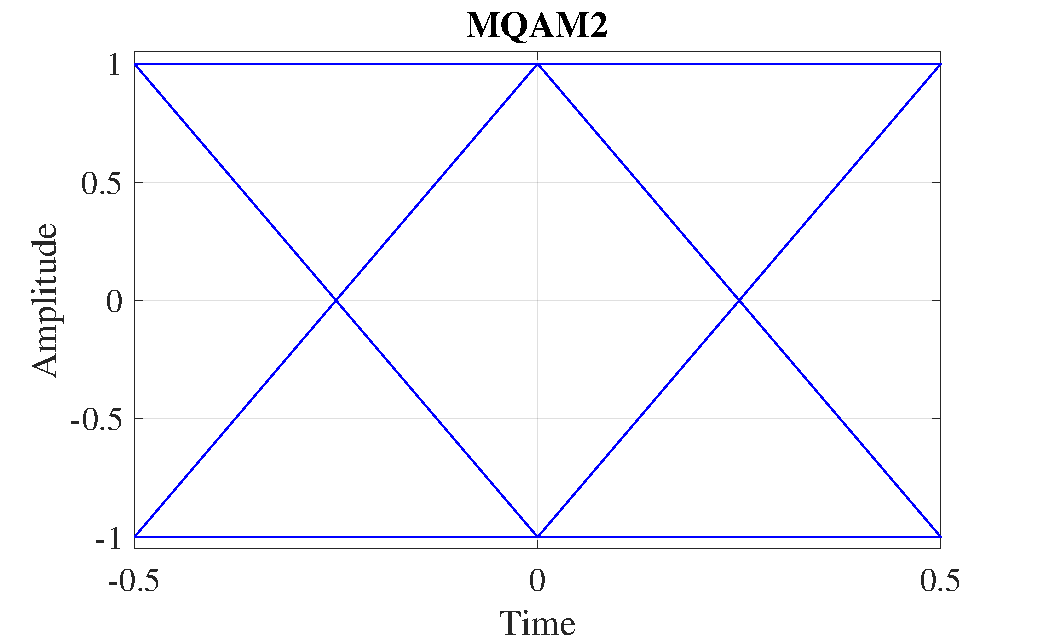
\includegraphics[width=\textwidth]{MQAM2}
\end{figure}

\subsection*{Sugestions for future improvement}

\end{document}